\section{Распространение ошибки и робастная калибровка}\label{sec:propagation}

\subsection{Аномалия: обрыв на $k=3$}

Кривые на рис.~\ref{fig:howmany} для M-O4 и его комбинаций немонотонны:
при $k=2$ рост PPL составляет 3.0\,\%, при $k=3$ "--- 27.0\,\%, а при $k=4$
"--- снова 11.3\,\%. У окна, SVD-LLM и отбора нейронов по готовым
активациям кривые гладкие. Поскольку $k=3$ совпадает с
$k_{\mathrm{sink}}$ (разд.~\ref{sec:results}), первая гипотеза
естественна: слой~3, в котором впервые возникает сток внимания,
усиливает ошибку, пришедшую из заменённых слоёв, а при $k=4$ его
собственная калибровка её компенсирует. Послойная диагностика
(рис.~\ref{fig:cliff}) эту гипотезу опровергает и указывает на другой
механизм.

\begin{figure}[t]
\centering
\figorpending{figures/cliff.pdf}{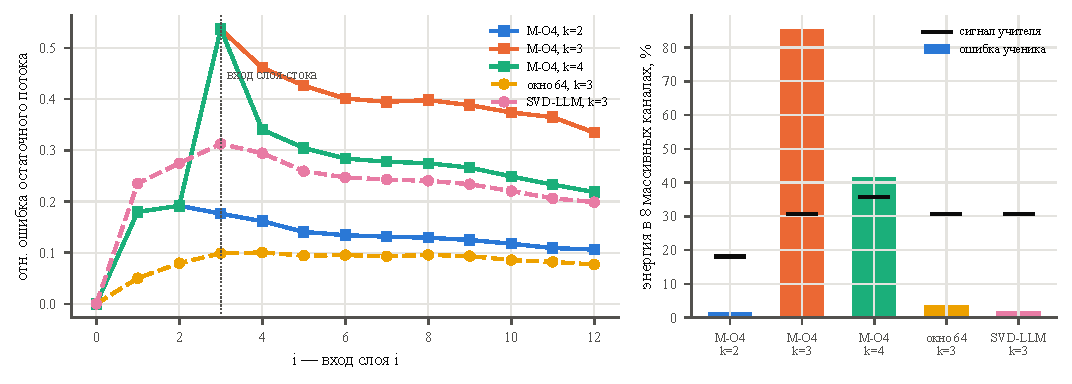
\includegraphics[width=\linewidth]{figures/cliff.pdf}}
\caption{Диагностика обрыва (Qwen3-0.6B, 8 окон по 1024 токена, позиции
$\ge 1$). Слева "--- относительная ошибка остаточного потока ученика на
входе каждого слоя. Справа "--- доля энергии ошибки на входе первого
незаменённого слоя, приходящаяся на 8 каналов массивной активации
(чёрточка "--- доля энергии сигнала учителя в тех же каналах).}
\label{fig:cliff}
\end{figure}

\subsection{Послойная диагностика}

Для каждой конфигурации мы сравниваем остаточный поток ученика и
учителя на входе каждого слоя (относительная ошибка по токенам, без
позиции~0). При $k=2$ ошибка после заменённых слоёв равна 0.18--0.19 и
далее монотонно убывает: каждый следующий слой гасит её с коэффициентом
около 0.9. При $k=3$ ошибка на входе слоя~3 равна 0.54, то есть скачок
происходит \emph{внутри заменённого слоя~2} (усиление 2.8), а слой~3
её не усиливает (коэффициент 0.86). Ошибка структурирована: 85\,\% её
энергии приходится на 8 каналов массивной активации, тогда как у
сигнала учителя в этих каналах 31\,\% энергии, у окна "--- 3.6\,\%, у
SVD-LLM "--- 1.7\,\%. Это сдвигает масштаб токенов именно в тех
координатах, по которым слой~3 отличает сток от остальных токенов:
средняя масса внимания на позиции~0 падает с 0.63 до 0.50, а средняя
абсолютная разность по позициям составляет 0.15. При $k=4$ калибровка
слоя~3 с компенсацией дрейфа снижает ошибку с 0.54 до 0.34, что и даёт
«восстановление» на кривой.

\subsection{Причина: одна строка калибровочной выборки}

MLP слоя~2 "--- тот блок, который создаёт массивную активацию: норма
остаточного потока на позиции~0 растёт с 19 до $\approx 7\,000$ именно
на его выходе. Калибровочная выборка состоит из 256 окон по 512
токенов, вырезанных из текста без начального токена. В $1.6\,\%$ таких
окон (33 из 2\,048 в большом пуле) модель образует сток не на позиции~0,
а на токене вроде <<0>>, <<8>> или <<=>> на позиции 1--2: выход MLP слоя~2
для него имеет норму $6\,400$--$7\,100$ при медиане $4.9$. В первых 32 тыс.
токенов нашей выборки такая строка одна и несёт $98.2\,\%$ энергии целей
$\sum_t\|y_t\|^2$; во всей выборке их около четырёх. Задача наименьших
квадратов для линейной поправки и предиктора нейронов M-O4 подгоняется
под эти строки, и ошибка в массивных каналах появляется у всех токенов.
Слои 0 и~1 не затронуты, потому что до слоя~2 массивной активации ещё
нет; в оценочных окнах таких токенов нет вовсе.

Ту же причину имеет неудача «корректоров»: поканальная, полная
($d\times d$), низкоранговая и ограниченная массивными каналами
линейные карты на входе слоя~3, подогнанные по сырым остаткам, не
уменьшают, а увеличивают рост PPL (с 27 до 35--45\,\%), поскольку те же
строки доминируют и в регрессорах.

\subsection{Формальная оценка: влияние одной строки}

Все рассматриваемые калибровки сводятся к гребневой регрессии
$W = (\Phi^\top\Phi + \lambda I)^{-1}\Phi^\top Y$ по строкам
$(\varphi_t, y_t)$, где $\varphi_t$ "--- признаки токена $t$ (вход блока с
единицей для смещения), $y_t$ "--- цель. Пусть строка $o$ добавлена к
набору $S$ остальных строк, $A = \Phi_S^\top\Phi_S + \lambda I$,
$W_S = A^{-1}\Phi_S^\top Y_S$ "--- решение без неё, $r_o = y_o -
\varphi_o^\top W_S$ "--- её невязка относительно этого решения и
$h_o = \varphi_o^\top A^{-1}\varphi_o$ "--- её рычаг.

\begin{proposition}\label{prop:leverage}
Решение с добавленной строкой равно
$W_{S\cup o} = W_S + \dfrac{A^{-1}\varphi_o\, r_o^\top}{1 + h_o}$, и для
любого токена $t$ изменение предсказания равно
\[
\Delta\hat y_t = \frac{c_{t}}{1 + h_o}\, r_o, \qquad c_t = \varphi_t^\top A^{-1}\varphi_o,
\]
так что $\|\Delta\hat y_t\| \le \dfrac{|c_t|}{1+h_o}\,\|r_o\|$, причём
$\Delta\hat y_t$ направлено вдоль $r_o$ для всех $t$ одновременно.
\end{proposition}

\begin{proof}
По формуле Шермана"--~Моррисона $(A + \varphi_o\varphi_o^\top)^{-1} =
A^{-1} - \frac{A^{-1}\varphi_o\varphi_o^\top A^{-1}}{1 + h_o}$. Подставляя в
$W_{S\cup o} = (A + \varphi_o\varphi_o^\top)^{-1}(\Phi_S^\top Y_S +
\varphi_o y_o^\top)$ и группируя слагаемые, получаем
$W_{S\cup o} - W_S = \frac{A^{-1}\varphi_o}{1+h_o}\,(y_o -
\varphi_o^\top W_S)^\top$; умножение слева на $\varphi_t^\top$ даёт
утверждение.
\end{proof}

Предложение объясняет два наблюдения и опровергает третье. Во-первых,
ошибка от строки с массивной активацией у \emph{всех} токенов лежит в
одном направлении $r_o$ "--- в каналах массивной активации (85\,\%
энергии ошибки на рис.~\ref{fig:cliff}). Во-вторых, её величина
пропорциональна $\|r_o\|$ и связи $c_t$. Измерения на слое~2
(табл.~\ref{tab:leverage}) подтверждают формулу: отклонение
$W_{S\cup o}-W_S$ от предсказания Шермана"--~Моррисона составляет
$4\cdot10^{-5}$, а предсказанная утечка в обычные токены "--- около половины
нормы их целей (медиана $53\,\%$ на 0.6B и $47\,\%$ на 1.7B). Третье
наблюдение "--- отсутствие обрыва на Qwen3-1.7B при том же выбросе
(норма $14\,355$) "--- предложение \emph{не} объясняет: утечка там такая же.
Разница в следующем слое: на 0.6B возмущение массивных каналов снижает
массу стока в слое~3 с $0.63$ до $0.50$, на 1.7B она не меняется
($0.589$ против $0.586$), и дальнейшие слои гасят ошибку. Иммунитет
большей модели "--- свойство устойчивости её стока, а не регрессии.
Величины $h_o$, $\|r_o\|$ и $\overline{|c_t|}$ измеримы \emph{до}
построения замены и дают априорный критерий опасности калибровочной
выборки.

\begin{table}[t]
\centering
\scriptsize
\setlength{\tabcolsep}{4pt}
\begin{tabular}{lrrrrrr}
\toprule
Модель, слой~2 & доля энергии $o$ & $h_o$ & $\|r_o\|$ & $\overline{|c_t|}$ & утечка (медиана / p90) & ошибка формулы \\
\midrule
Qwen3-0.6B & 26\,\% & 0.094 & 5\,250 & $5.6\cdot10^{-4}$ & 53\,\% / 112\,\% & $4\cdot10^{-5}$ \\
Qwen3-1.7B & 27\,\% & 0.128 & 9\,801 & $6.2\cdot10^{-4}$ & 47\,\% / 100\,\% & $4\cdot10^{-5}$ \\
\bottomrule
\end{tabular}
\caption{Влияние строки с максимальной нормой цели в калибровке (131 тыс.
токенов) на гребневую регрессию для MLP слоя~2: доля энергии целей, рычаг,
невязка, средняя связь с обычными токенами, предсказанная относительная
утечка в их предсказания и относительная ошибка формулы
Шермана"--~Моррисона. Для слоёв 0, 1 и 3 утечка не превышает $0.5\,\%$.}
\label{tab:leverage}
\end{table}

\subsection{Управляемый эксперимент}

Если причина "--- состав калибровки, обрыв должен включаться и
выключаться числом отравленных окон. Мы просканировали пул из 2\,048
окон, пометили окна с массивной активацией на позиции $\ge 1$ и
собирали калибровку из 256 окон с $n = 0, 1, 4, 16$ отравленными
(рис.~\ref{fig:toggle}). На Qwen3-0.6B наивный M-O4 при $k=3$ даёт
4.2\,\% при $n = 0$ и $n = 1$, 23.9\,\% при $n = 4$ и 379\,\% при $n = 16$;
робастная калибровка при $n = 16$ возвращает 4.1\,\%. На Qwen3-1.7B все
дозы дают 1.6--1.7\,\%. Зависимость от дозы причинная, порог "--- между
одним и четырьмя окнами из 256, и стандартная выборка с $\approx 4$
отравленными окнами попадает ровно в область обрыва.

\begin{figure}[t]
\centering
\figorpending{figures/toggle.pdf}{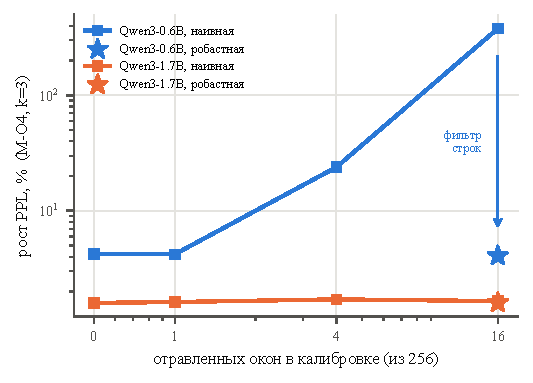
\includegraphics[width=0.55\linewidth]{figures/toggle.pdf}}
\caption{Рост PPL наивно откалиброванного M-O4 ($k=3$) в зависимости от
числа отравленных окон в калибровочной выборке из 256 окон; звёздочки "---
робастная калибровка при $n=16$.}
\label{fig:toggle}
\end{figure}

\subsection{Нейроны стока}

Массивную активацию позиции~0 создают единичные нейроны MLP слоя~2:
на Qwen3-0.6B пять нейронов дают 90\,\% вклада, на Qwen3-1.7B "--- один
нейрон 94\,\% (табл.~\ref{tab:sink}). Их удаление во всех позициях
уничтожает сток (норма $h_0$ падает с $6\,897$ до $429$ и с $14\,701$ до
$225$) и разрушает модель: $+54\,\%$ и $+231\,\%$ PPL. Удаление тех же
нейронов только на позициях $t \ge 1$ стоит $0.3\,\%$ и $0.0\,\%$, случайных
нейронов "--- ничего. Это объясняет, почему любой отбор нейронов в ранних
слоях обязан либо считать позицию~0 точно (как все наши MLP-замены), либо
защищать эти нейроны явно: в робастной статистике, исключающей позицию~0
и выбросы, нейрон стока невидим "--- вся его энергия сосредоточена именно
там. Полный A3 без точной позиции~0 с робастным отбором терял его и давал
$+556\,\%$ на 1.7B; с точной позицией~0 "--- $46\,\%$, как и наивный.
Нейроны стока "--- MLP-аналог <<супервесов>>~\cite{yu2024superweights}:
несколько параметров, без которых модель не работает.

\begin{table}[t]
\centering
\scriptsize
\setlength{\tabcolsep}{3pt}
\IfFileExists{tables/sink.tex}{\begin{tabular}{lcccrrrr}
\toprule
Модель & слой & нейронов & доля вклада в поз.~0 & \multicolumn{2}{c}{удалить везде} & удалить при $t\ge1$ & случайные \\
 & & & & $\Delta$PPL & $\|h_0\|$ после слоя & $\Delta$PPL & $\Delta$PPL \\
\midrule
Qwen3-0.6B & 2 & 5 & 90\% & +54.4\% & 429 & +0.3\% & -0.0\% \\
Qwen3-1.7B & 2 & 1 & 94\% & +230.9\% & 225 & +0.0\% & -0.0\% \\
\bottomrule
\end{tabular}
}{\textcolor{red}{[ожидает прогона]}}
\caption{Нейроны стока в слое $k_{\mathrm{sink}}-1$ и абляции (8 окон по
1024 токена): удаление во всех позициях, только при $t\ge1$ (позиция~0
точно) и такого же числа случайных нейронов.}
\label{tab:sink}
\end{table}

\subsection{Робастная калибровка}

Исправление детерминировано и бесплатно: из всех сумм по токенам
исключаются строки с $\|y_t\| > \tau \operatorname{med}_t \|y_t\|$,
$\tau = 10$ (правило не задевает ни одной обычной строки: доля токенов с
$\|z\|>10\,\mathrm{med}$ сверх выбросов равна нулю на обеих моделях), а в
критериях отбора нейронов "--- ещё и позиция~0 при точном её вычислении.
С робастной калибровкой обрыв исчезает (рис.~\ref{fig:howmany}): рост
PPL у M-O4 при $k=3$ составляет 4.7\,\% вместо 27.0\,\%, при $k=4$ "---
6.4 вместо 11.3, при $k=6$ "--- 8.7 вместо 13.0, при $k=8$ "--- 11.0 вместо
14.9, при $k=12$ "--- 14.7 вместо 19.3; у комбинации окно\,+\,M-O4 "--- 5.2,
7.5, 10.1, 13.6 и 22.2\,\% вместо 29.6, 13.1, 14.9, 18.1 и 27.6. Выигрыш
виден и на бенчмарках при $k=3$: средняя точность по семи задачам у
M-O4 растёт с 44.4 до 54.6\,\% при 54.9\,\% у исходной модели, у
окна\,+\,M-O4 "--- с 46.2 до 54.3\,\%. Та же поправка спасает M-O1 с
25\,\% точных нейронов (54.2 $\to$ 10.2\,\%) и табличную замену M-O2
(30.6 $\to$ 12.2\,\%). Робастная замкнутая форма оказывается сильнее
наивной калибровки с последующей дистилляцией: 300 шагов AdamW снижают
ошибку M-O1 лишь до 12.5\,\%.

\paragraph{Кого ловушка не касается.} Табл.~\ref{tab:robust} сравнивает
наивную и робастную калибровку для всех методов. Опубликованные методы
не страдают: SVD-LLM (12.8 против 12.6\,\%), ASVD (38.5 против 38.7\,\%)
и A3 (9.9 против 9.9\,\%) используют статистики для \emph{ранжирования}
или \emph{отбеливания}, а не как цели регрессии. Так, в матрице
$X^\top X$ входов down-проекции слоя~2, которую отбеливает SVD-LLM,
позиция~0 даёт $98.4\,\%$ следа, а среди позиций $\ge1$ один токен "---
$25.6\,\%$; но доминирующее направление лишь получает собственную
сингулярную компоненту и сохраняется при усечении. Страдают методы,
решающие задачу наименьших квадратов с целями в остаточном потоке: наши
M-O1, M-O2, M-O4 и, как показано ниже, корректоры на границе блоков.
Проверка на родных настройках SVD-LLM и ASVD (сжатие 10 и 20\,\%,
калибровка 256 окон по 2048 токенов, $k=3$) подтверждает это: наивная и
робастная статистики дают одинаковый результат (SVD-LLM 4.7/4.7 и
3.2/3.3\,\% на 0.6B, 1.5/1.5 и 0.9/0.9\,\% на 1.7B; ASVD 9.5/9.5 и 5.5/5.5,
4.9/4.9 и 3.0/3.0\,\%). Заметим, что при 20\,\% сжатия SVD-LLM стоит
столько же, сколько M-O4 при 75\,\% экономии MLP.

\begin{table}[t]
\centering
\small
\IfFileExists{tables/robust.tex}{\begin{tabular}{lrrrr}
\toprule
Метод & \multicolumn{2}{c}{наивная калибровка} & \multicolumn{2}{c}{робастная} \\
 & $\Delta$PPL & KL & $\Delta$PPL & KL \\
\midrule
SVD-LLM 50\% & 12.8\% & 0.138 & 12.6\% & 0.137 \\
ASVD 50\% & 38.5\% & 0.359 & 38.7\% & 0.361 \\
A3 FFN 50\% & 9.9\% & 0.114 & 9.9\% & 0.113 \\
A3 (блок) & 49.2\% & 0.433 & 49.5\% & 0.435 \\
M-O2: таблица по токену & 30.6\% & 0.288 & 12.2\% & 0.141 \\
M-O1: линейный + 25\% & 57.7\% & 0.480 & 10.2\% & 0.115 \\
M-O4: предиктор 25\% & 27.0\% & 0.268 & 4.7\% & 0.056 \\
Окно + M-O4 & 29.6\% & 0.286 & 5.2\% & 0.065 \\
\bottomrule
\end{tabular}
}{\textcolor{red}{[ожидает прогона]}}
\caption{Наивная и робастная калибровка при $k=k_{\mathrm{sink}}$
(Qwen3-0.6B, WikiText-2, 32 окна). Методы ранжирования и отбеливания
(SVD-LLM, ASVD, A3) не меняются; регрессионные замены меняются в
разы.}
\label{tab:robust}
\end{table}

\paragraph{Корректор на границе.} Оператор выравнивания активаций на
границе заменённого блока (ReplaceMe~\cite{shopkhoev2025replaceme},
Ghosted Layers~\cite{yun2026ghosted}) "--- та же регрессия. Подогнанный
наивно, он ухудшал наивный M-O4 (разд.~выше); подогнанный с исключением
строк-выбросов, он исправляет его: 27.0 $\to$ 4.8\,\% для полной карты
$d\times d$ и 4.7\,\% для карты, корректирующей только 8 каналов массивной
активации. На робастно откалиброванном M-O4 корректор ничего не добавляет
(4.7 $\to$ 4.7\,\%). Восьми каналов достаточно "--- прямое подтверждение
того, что вся ошибка ловушки лежит в направлении $r_o$.

\subsection{Стоки на токенах: второе семейство}
\label{sec:tokensinks}

У моделей архитектуры Llama правило <<сток "--- позиция~0>> оказывается
частным случаем более общего. На SmolLM2-1.7B массивную активацию
(норма $\approx 2\,900$ при медиане 33 после слоя~1) создаёт один нейрон
MLP слоя~1 (№\,4987, 68--89\,\% вклада) на токене <<\,the\,>> (а также на
первых кавычке и двойном переводе строки) в \emph{любой} позиции; сток
позиции~0 появляется лишь после слоя~7, и до него поздние слои используют
как стоки именно эти массивные токены. На Llama-3.2-1B массивную
активацию позиции~0 создают 12 нейронов MLP слоя~1 (90\,\% вклада);
их удаление во всех позициях стоит $+1\,353\,\%$ PPL, только при $t\ge1$
"--- $0.9\,\%$, у SmolLM2 64 нейрона слоя~7 (86\,\%) "--- $+2\,190$ и
$0.2\,\%$. Механизм тот же, что у Qwen3, но триггер иной.

Следствий два, и оба меняют замены. Во-первых, калиброванные замены MLP
без защиты рушатся даже с робастным фильтром строк по норме входа, потому
что массивные строки сидят в \emph{целях} регрессии на обычных токенах:
на SmolLM2 при $k=2$ M-O4 даёт $+123\,\%$, окно\,+\,M-O4 "--- $+612\,\%$.
Лечение детерминировано: нейроны стока находятся по калибровке априори
(токены с $\|\mathrm{MLP}(x)\|>20\,\mathrm{med}$, нейроны, покрывающие
90\,\% их вклада), всегда остаются в маске предиктора и отборе, у SVD
выносятся из факторизации и добавляются точно, а строки с большой
невязкой регрессии исключаются из подгонки (невязка нужна потому, что
окно внимания меняет набор токенов, становящихся массивными). После
этого M-O4 стоит $11.3\,\%$, окно\,+\,M-O4 "--- $13.9\,\%$, гребневая
замена "--- $15.3\,\%$; SVD-LLM остаётся непригодным (123\,\%). На
Qwen3 те же правки не меняют ни одного числа (4.7, 12.7 и 5.2\,\% при
$k=3$ на 0.6B), потому что там нейроны стока действуют только в позиции~0,
которая и так считается точно. Во-вторых, окно внимания должно хранить
массивные ключи в любой позиции: ключ считается стоком, если отношение
пика его каналов к среднему после RMSNorm превышает удвоенную медиану по
последовательности (априорное правило без калибровки). На SmolLM2 это
даёт $2.0\,\%$ вместо $13.7\,\%$ при $k=3$, $3.5$ вместо $62.4\,\%$ при
$k=6$ и $4.4$ вместо $64.1\,\%$ при $k=8$ ценой 0.2--4.4\,\% лишних
ключей; на Llama-3.2-1B "--- $2.8$ вместо $13.1\,\%$ при $k=2$; на Qwen3
ничего не портит: на 1.7B при $k=1..8$ кривая совпадает с позиционным стоком или чуть ниже
(5.5 вместо 5.7\,\% при $k=8$) при 0--0.1\,\% лишних ключей. Дозовый эксперимент на этом
семействе ловушку не включает (33.2--33.6\,\% при 0--16 отравленных окнах
на SmolLM2, 15.6--15.8\,\% на Llama-3.2-1B): отравление здесь не в
составе калибровки, а в самих данных, где массивные токены есть всегда.

\subsection{Вывод}

Любая калибровка в замкнутой форме, которая накапливает суммы по
токенам "--- гребневая регрессия, отбор нейронов по $\sum_t z_t^2$,
PCA входов "--- должна исключать позицию~0 и токены с массивной
активацией. Иначе ошибка приближения ложится в каналы стока и разрушает
механизм внимания ниже по потоку, причём ровно на том слое, где
появляется сток. Для квантования аналогичная роль каналов-выбросов
известна~\cite{yuan2023asvd}; здесь показано, что при структурной
замене блоков опасен не канал, а единичный токен в данных. В общем виде
правило звучит так: сток "--- это массивная активация, где бы она ни
возникла; позиция~0 у Qwen3 "--- частный случай, токен <<the>> у SmolLM2 "---
другой, и замена обязана сохранять и нейроны, создающие такие активации,
и ключи, которые их несут.
